%-----------------------------------------------------------------------------------------------------------------------------------------------%
%	The MIT License (MIT)
%
%	Copyright (c) 2015 Jan Küster
%
%	Permission is hereby granted, free of charge, to any person obtaining a copy
%	of this software and associated documentation files (the "Software"), to deal
%	in the Software without restriction, including without limitation the rights
%	to use, copy, modify, merge, publish, distribute, sublicense, and/or sell
%	copies of the Software, and to permit persons to whom the Software is
%	furnished to do so, subject to the following conditions:
%	
%	THE SOFTWARE IS PROVIDED "AS IS", WITHOUT WARRANTY OF ANY KIND, EXPRESS OR
%	IMPLIED, INCLUDING BUT NOT LIMITED TO THE WARRANTIES OF MERCHANTABILITY,
%	FITNESS FOR A PARTICULAR PURPOSE AND NONINFRINGEMENT. IN NO EVENT SHALL THE
%	AUTHORS OR COPYRIGHT HOLDERS BE LIABLE FOR ANY CLAIM, DAMAGES OR OTHER
%	LIABILITY, WHETHER IN AN ACTION OF CONTRACT, TORT OR OTHERWISE, ARISING FROM,
%	OUT OF OR IN CONNECTION WITH THE SOFTWARE OR THE USE OR OTHER DEALINGS IN
%	THE SOFTWARE.
%	
%
%-----------------------------------------------------------------------------------------------------------------------------------------------%


%============================================================================%
%
%	DOCUMENT DEFINITION
%
%============================================================================%

%we use article class because we want to fully customize the page and dont use a cv template
\documentclass[10pt,A4]{article}	


%----------------------------------------------------------------------------------------
%	ENCODING
%----------------------------------------------------------------------------------------

%we use utf8 since we want to build from any machine
\usepackage[utf8]{inputenc}		

%----------------------------------------------------------------------------------------
%	LOGIC
%----------------------------------------------------------------------------------------

% provides \isempty test
\usepackage{xifthen}

%----------------------------------------------------------------------------------------
%	FONT
%----------------------------------------------------------------------------------------

% some tex-live fonts - choose your own

%\usepackage[defaultsans]{droidsans}
%\usepackage[default]{comfortaa}
%\usepackage{cmbright}
%\usepackage[default]{raleway}
%\usepackage{fetamont}
\usepackage[default]{gillius}
%\usepackage[light,math]{iwona}
%\usepackage[thin]{roboto} 

% set font default
\renewcommand*\familydefault{\sfdefault} 	
\usepackage[T1]{fontenc}

% more font size definitions
\usepackage{moresize}		

\usepackage{fontawesome5}
\usepackage{tikz}
%----------------------------------------------------------------------------------------
%	PAGE LAYOUT  DEFINITIONS
%----------------------------------------------------------------------------------------

%debug page outer frames
%\usepackage{showframe}			


%define page styles using geometry
\usepackage[a4paper]{geometry}		

% for example, change the margins to 2 inches all round
\geometry{top=1cm, bottom=-.6cm, left=0.4cm, right=1cm} 	


%less space between header and content
\setlength{\headheight}{-5pt}		


%customize entries left, center and right
%\lhead{}
%\chead{ \small{Oren Rozen  $\cdot$ Consultant and Software Engineer $\cdot$  Bremen, Germany  $\cdot$  \textcolor{sectcol}{\textbf{info@jankuester.com}}  $\cdot$ +49 176 313 *** **}}
%\rhead{}


%indentation is zero
\setlength{\parindent}{0mm}

%----------------------------------------------------------------------------------------
%	TABLE /ARRAY DEFINITIONS
%---------------------------------------------------------------------------------------- 

%for layouting tables
\usepackage{multicol}			
\usepackage{multirow}

%extended aligning of tabular cells
\usepackage{array}

\newcolumntype{x}[1]{%
>{\raggedleft\hspace{0pt}}p{#1}}%


%----------------------------------------------------------------------------------------
%	GRAPHICS DEFINITIONS
%---------------------------------------------------------------------------------------- 

%for header image
\usepackage{graphicx}

%for floating figures
\usepackage{wrapfig}
\usepackage{float}
%\floatstyle{boxed} 
%\restylefloat{figure}

%for drawing graphics		
\usepackage{tikz}				
\usetikzlibrary{shapes, backgrounds,mindmap, trees}


%----------------------------------------------------------------------------------------
%	Color DEFINITIONS
%---------------------------------------------------------------------------------------- 
\usepackage{transparent}
\usepackage{color}

%accent color
\definecolor{complcol}{RGB}{250,150,10}

%dark background color
\definecolor{bgcol}{RGB}{110,110,110}

%light background / accent color
\definecolor{softcol}{RGB}{225,225,225}

\definecolor{sectcol}{RGB}{0,120,150}


%Package for links, must be the last package used
\usepackage[hidelinks]{hyperref}

%============================================================================%
%
%
%	DEFINITIONS
%
%
%============================================================================%

% returns minipage width minus two times \fboxsep
% to keep padding included in width calculations
\newcommand{\mpwidth}{\linewidth-\fboxsep-\fboxsep}
	

%----------------------------------------------------------------------------------------
% 	ARROW GRAPHICS in Tikz
%----------------------------------------------------------------------------------------

% a six pointed arrow poiting to the left
\newcommand{\tzlarrow}{(0,0) -- (0.2,0) -- (0.3,0.2) -- (0.2,0.4) -- (0,0.4) -- (0.1,0.2) -- cycle;}	

% include the left arrow into a tikz picture
% param1: fill color
%
\newcommand{\larrow}[1]
{\begin{tikzpicture}[scale=0.58]
	 \filldraw[fill=#1!100,draw=#1!100!black]  \tzlarrow
 \end{tikzpicture}
}

% a six pointed arrow poiting to the right
\newcommand{\tzrarrow}{ (0,0.2) -- (0.1,0) -- (0.3,0) -- (0.2,0.2) -- (0.3,0.4) -- (0.1,0.4) -- cycle;}

% include the right arrow into a tikz picture
% param1: fill color
%
\newcommand{\rarrow}
{
\begin{tikzpicture}[scale=0.7]
	\filldraw[fill=sectcol!100,draw=sectcol!100!black] \tzrarrow
 \end{tikzpicture}
}

%----------------------------------------------------------------------------------------
%	custom sections
%----------------------------------------------------------------------------------------

% create a coloured box with arrow and title as cv section headline
% param 1: section title
%
\newcommand{\cvsection}[1]
{
\colorbox{sectcol}{\mystrut \makebox[1\mpwidth][l]{
\larrow{bgcol} \hspace{-8pt} \larrow{bgcol} \hspace{-8pt} \larrow{bgcol} \textbf{\textcolor{white}{\uppercase{#1}}}\hspace{4pt}
}}\\
}

% create a coloured arrow with title as cv meta section section
% param 1: meta section title
%
\newenvironment{metasection}[1] {
	\vspace{9pt}
	\begin{center}
		\textcolor{white}{\large{\uppercase{#1}}}\\
	\normalsize
	\parbox{0.7\mpwidth}{\textcolor{white}	\hrule}
}{\end{center}}

%----------------------------------------------------------------------------------------
%	 CV EVENT
%----------------------------------------------------------------------------------------

% creates a stretched box as cv entry headline followed by two paragraphs about 
% the work you did
% param 1:	event time i.e. 2014 or 2011-2014 etc.
% param 2:	event name (what did you do?)
% param 3:	institution (where did you work / study)
% param 4:	what was your position
% param 5:	some words about your contributions
%
\newcommand{\cvevent}[7]
{
	\begin{tabular*}{1\mpwidth}{p{0.55\mpwidth}  x{0.42\mpwidth}}
 	\textcolor{black}{\textbf{#2}} & \textcolor{complcol}{#3}, \textcolor{bgcol}{#1} 

	\end{tabular*}
\vspace{-12pt}
\textcolor{softcol}{\hrule}
	\begin{itemize}
		\setlength\itemsep{3pt}
		\item[\larrow{softcol}]  #4
		\item[\larrow{softcol}]  #5
		\item[\larrow{softcol}]  #6
		\item[\larrow{softcol}]  #7
	\end{itemize}
\vspace{-6pt}

}
\newcommand{\cveventA}[3]
{
	\begin{tabular*}{1\mpwidth}{p{0.55\mpwidth}  x{0.42\mpwidth}}
 	\textcolor{black}{\textbf{#2}} & \textcolor{complcol}{#3}, \textcolor{bgcol}{#1} 

	\end{tabular*}

}


\newcommand{\expertiseB}[5]
{
	\begin{tabular*}{1\mpwidth}{p{0.55\mpwidth}  x{0.42\mpwidth}}
 	\textcolor{black}{\textbf{#2}} & \textcolor{bgcol}{#1} 
	\end{tabular*}
	\textcolor{softcol}{\hrule}
	\vspace{-3pt}
	\begin{itemize}
		\setlength\itemsep{3pt}
		\item[\larrow{softcol}]  #3
		\item[\larrow{softcol}]  #4
	\end{itemize}
	\vspace{-6pt}
}

\newcommand{\expertiseA}[5]
{
	\begin{tabular*}{1\mpwidth}{p{0.55\mpwidth}  x{0.42\mpwidth}}
 	\textcolor{black}{\textbf{#2}} & \textcolor{bgcol}{#1} 
	\end{tabular*}
	\textcolor{softcol}{\hrule}
	\vspace{-3pt}
	\begin{itemize}
		\item[\larrow{softcol}]  #3
	\end{itemize}
	\vspace{-6pt}
}

% creates a stretched box as 
\newcommand{\cveventmeta}[2]
{
	\mbox{\mystrut \hspace{87pt}\textit{#1}}\\
	#2
}

%----------------------------------------------------------------------------------------
% CUSTOM STRUT FOR EMPTY BOXES
%----------------------------------------- -----------------------------------------------
\newcommand{\mystrut}{\rule[-.3\baselineskip]{0pt}{\baselineskip}}

%----------------------------------------------------------------------------------------
% CUSTOM LOREM IPSUM
%----------------------------------------------------------------------------------------
\newcommand{\lorem}
{Lorem ipsum dolor sit amet, consectetur adipiscing elit. Donec a diam lectus.}


% use to vertically center content
% credits to: http://tex.stackexchange.com/questions/7219/how-to-vertically-center-two-images-next-to-each-other
\newcommand{\vcenteredinclude}[1]{\begingroup
\setbox0=\hbox{\includegraphics{#1}}%
\parbox{\wd0}{\box0}\endgroup}

% use to vertically center content
% credits to: http://tex.stackexchange.com/questions/7219/how-to-vertically-center-two-images-next-to-each-other
\newcommand*{\vcenteredhbox}[1]{\begingroup
\setbox0=\hbox{#1}\parbox{\wd0}{\box0}\endgroup}

%----------------------------------------------------------------------------------------
%	ICON-SET EMBEDDING
%---------------------------------------------------------------------------------------- 

% at this point we simplify our icon-embedding by simply referring to a set of png images.
% if you find a good way of including svg without conflicting with other packages you can
% replace this part
\newcommand{\icon}[3]{\makebox(#2, #2){\textcolor{#3}{\csname fa#1\endcsname}}}	%icon shortcut
\newcommand{\icontext}[4]{ 						%icon with text shortcut
	\vcenteredhbox{\icon{#1}{#2}{#4}} \vcenteredhbox{\textcolor{#4}{#3}}
}
\newcommand{\iconhref}[5]{ 						%icon with website url
    \vcenteredhbox{\icon{#1}{#2}{#5}} \href{#4}{\textcolor{#5}{#3}}
}

\newcommand{\iconemail}[5]{ 						%icon with email link
    \vcenteredhbox{\icon{#1}{#2}{#5}} \href{mailto:#4}{\textcolor{#5}{#3}}
}



%============================================================================%
%
%
%
%	DOCUMENT CONTENT
%
%
%
%============================================================================%
\begin{document}
\fcolorbox{white}{white}{\begin{minipage}[c][0.95\textheight][t]{0.69\linewidth}


%---------------------------------------------------------------------------------------
%	TITLE HEADLINE
%----------------------------------------------------------------------------------------
\vspace{-3pt}
% use this for multiple words like working titles etc.
%\hspace{-0.25\linewidth}\colorbox{bgcol}{\makebox[1.5\linewidth][c]{\hspace{46pt}\HUGE{\textcolor{white}{\uppercase{M.Sc. Jan Küster}} } \textcolor{sectcol}{\rule[-1mm]{1mm}{0.9cm}} \parbox[b]{5cm}{   \large{ \textcolor{white}{{IT Consultant}}}\\
% \large{ \textcolor{white}{{JS Fullstack Engineer}}}}
%}}

% use this for single words, e.g. CV or RESUME etc.
\colorbox{bgcol}{\makebox[\mpwidth][c]{\HUGE{\textcolor{white}{\uppercase{Oren Rozen}} } \textcolor{sectcol}{\rule[-1mm]{1mm}{0.9cm}} \HUGE{\textcolor{white}{\uppercase{Resume}} } }}

%----------------------------------------------------------------------------------------
%	HEADER IMAGE
%----------------------------------------------------------------------------------------


%\hspace{-1.6cm}
%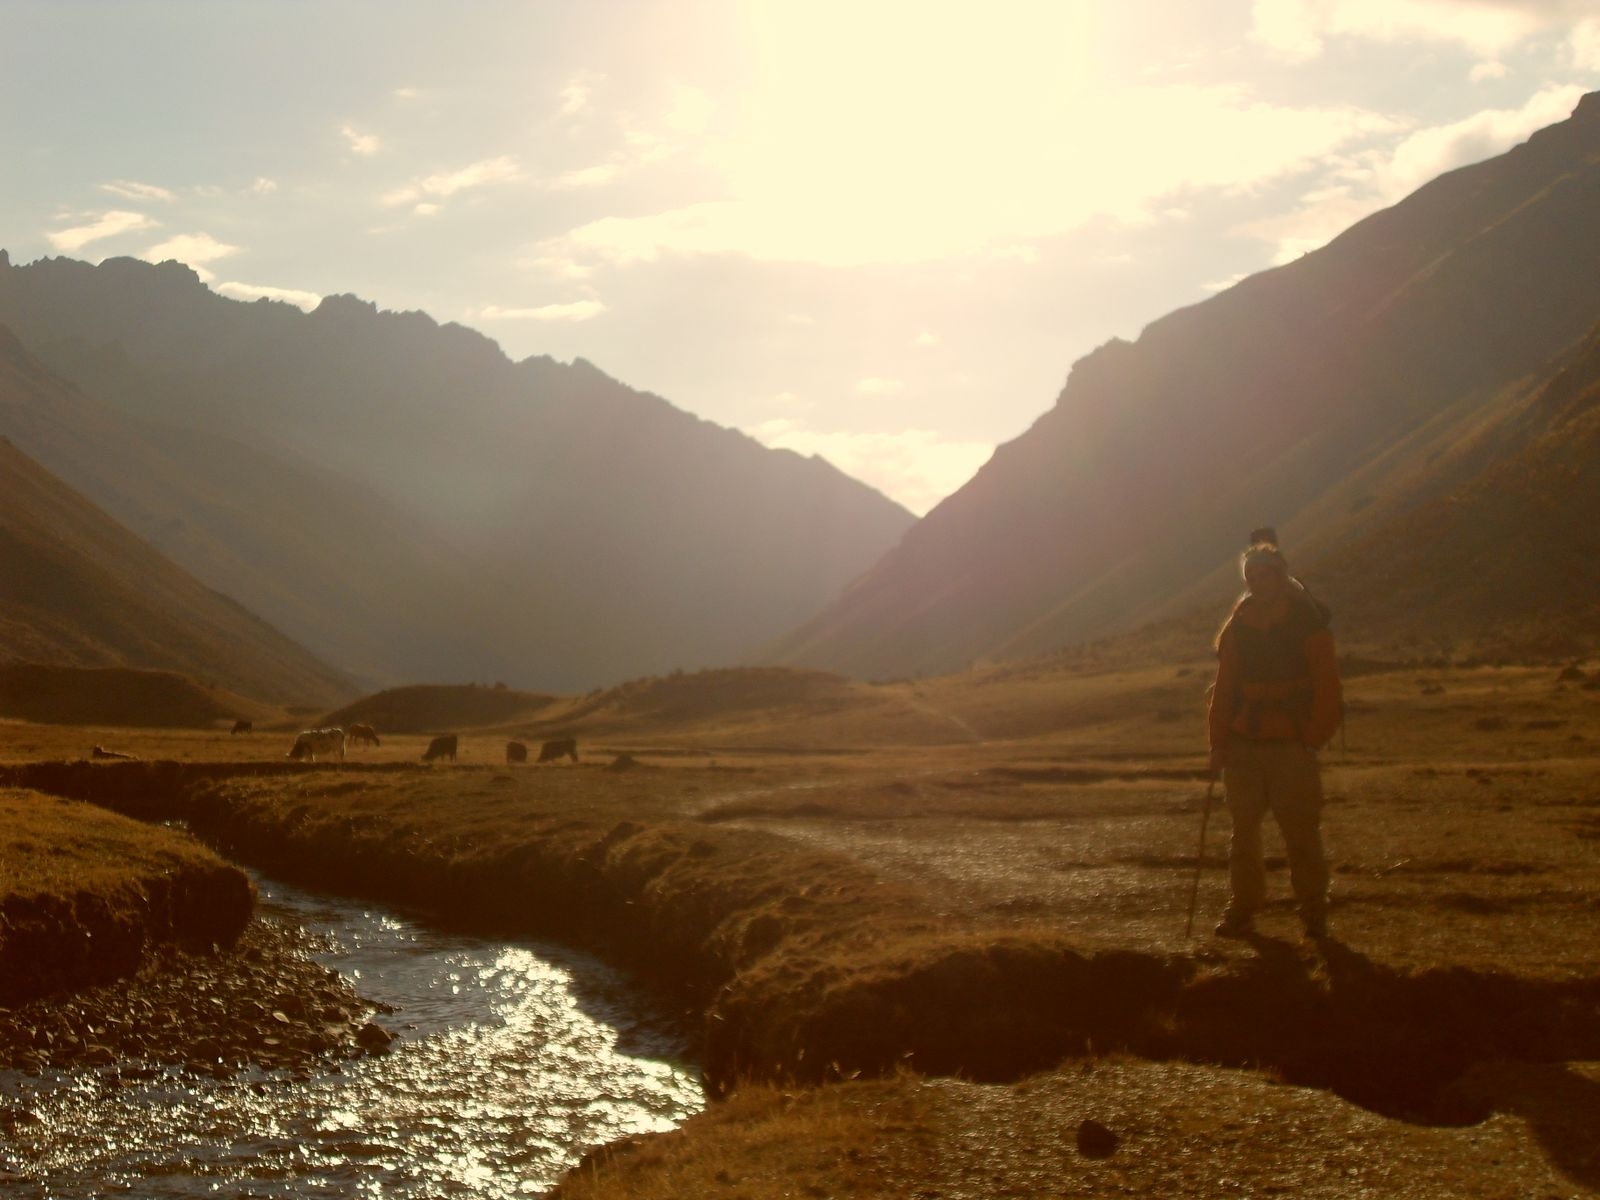
\includegraphics[trim= 0 250 0 270,clip,width=1\linewidth+3.1cm]{myfoto.jpg}	%trimming relative to image size!
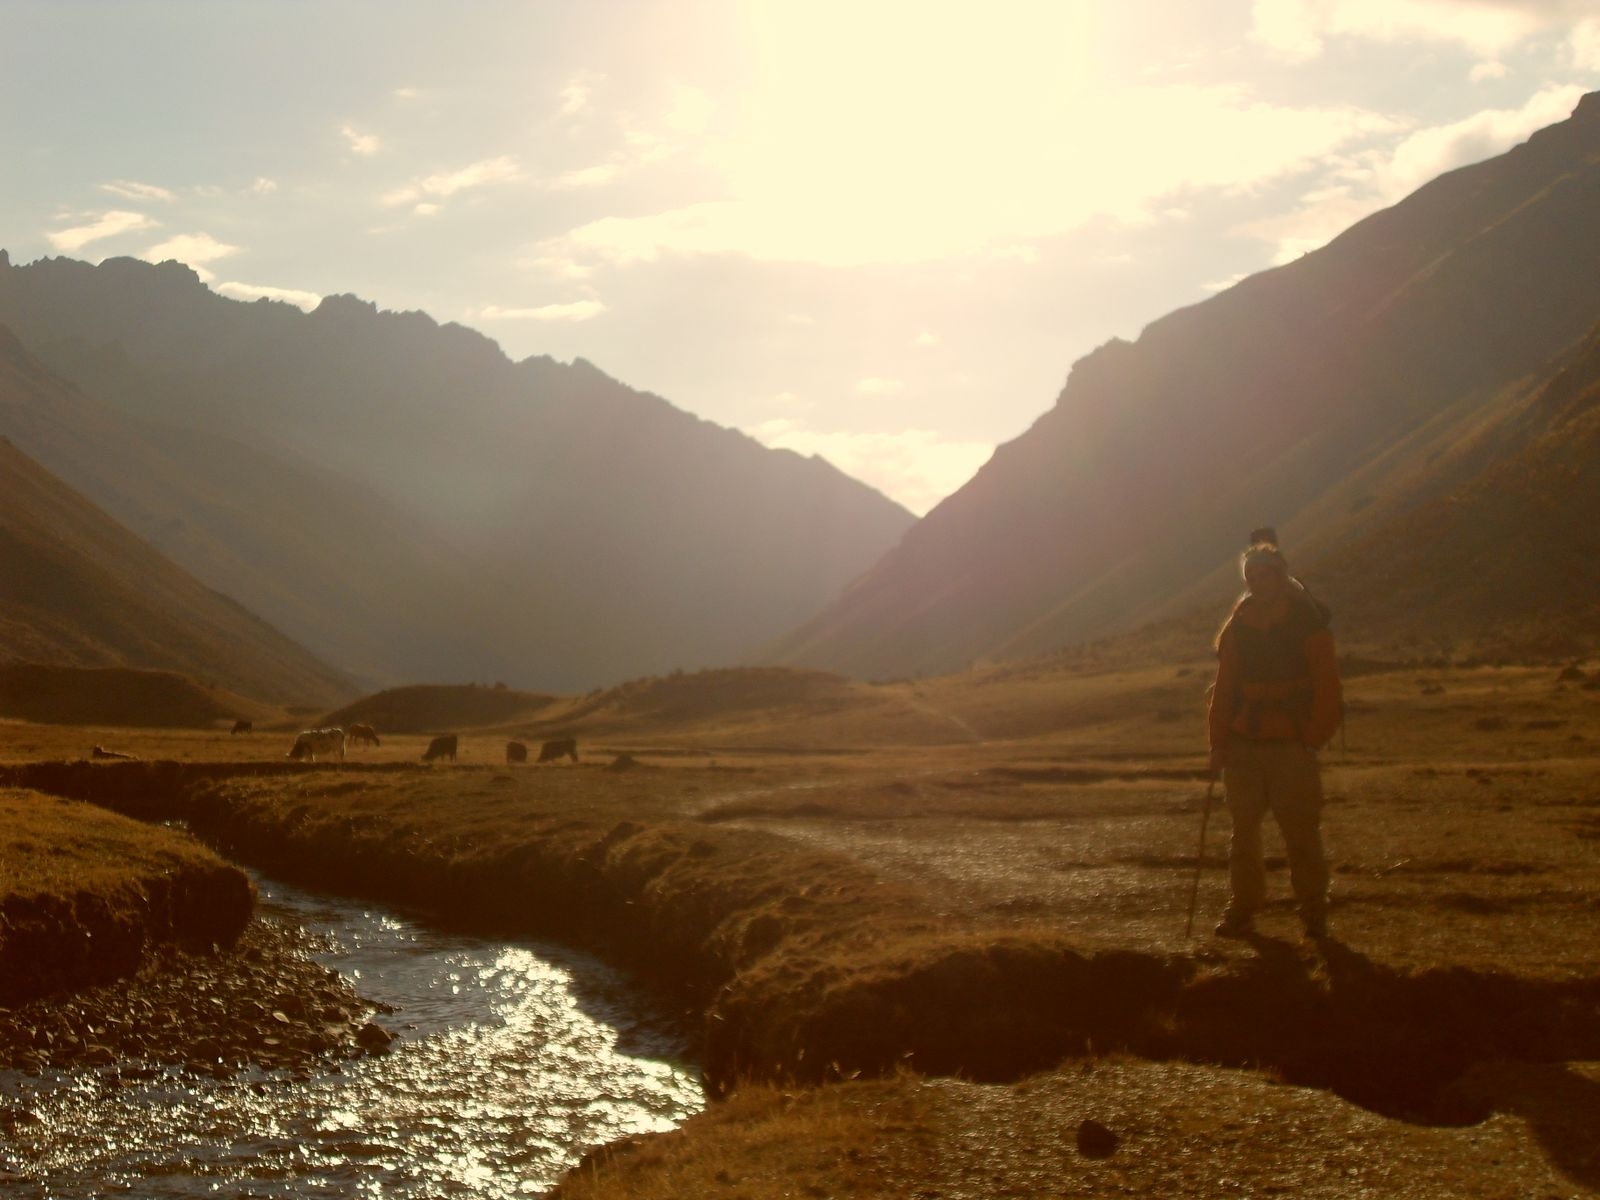
\includegraphics[trim= 100 170 0 275, clip ,width=\linewidth]{myfoto.jpg}	%trimming relative to image size
%---------------------------------------------------------------------------------------
%	SUMMARY
%----------------------------------------------------------------------------------------
\vspace{-130pt}

\begin{center}
	\hspace{-80pt}
	% \transparent{0.1}%
	\transparent{0.1}%
	\colorbox{bgcol}{
		% \transparent{0.1}%
		\parbox{0.6\linewidth}{
			\textcolor{white}{%
			" I am passionate about creating and designing software 
			that helps people and businesses focus on what's most important to them."
			}
		}
	}
\end{center}

\vspace{60pt}


% \transparent{0.85}%
% \vspace*{-130pt}
% \hspace{0.1\linewidth}
% 	\put(10,-100) {\colorbox{bgcol}{
% 	\parbox{0.5\linewidth}{
% 		\transparent{1}%
% 		\begin{center}
% 		\textcolor{white}{" I am passionate about creating and designing software that helps people and businesses focus on what's most important to them."}
% 		\end{center}
% 	}
% }
% 	}
% \vspace{68pt}

%============================================================================%
%
%	CV SECTIONS AND EVENTS (MAIN CONTENT)
%
%============================================================================%

%---------------------------------------------------------------------------------------
%	STATUS
%----------------------------------------------------------------------------------------
\cvsection{About Me}

I have been working as a developer for a company located in Panama that customizes and gives support for SAP B1. I’ve created Applications/Servers/Mobile apps to enhance the usage and efficiency of our clients using SAP B1 (Retail stores, Suppliers, Hotels, etc.) The primary language we use is C\#. I created state-of-the-art tools for our developers to easily implement SAP B1/SQL/DBs integrations for our clients.
I have a strong passion for functional programming, and I am using it as my primary programming technique.

\vspace{7pt}

%---------------------------------------------------------------------------------------
%	EXPERIENCE
%----------------------------------------------------------------------------------------

\cvsection{Expertise}

%
\vspace{-3pt}
\expertiseB{10 years experience}{C\#}
{
	Developed and managed tools that help our developers to be more productive in creating business integrations (SAP B1, SQL, ReavenDB, DSL).
}
{
	Maintain a substantial code base for fiscal printers implementation.
}

\expertiseA{5 years experience}{Java}
{
	Used Java to create plugins for Jira and Confluence, which handles the company workflows for finance, sales, consulting, and software development departments. 
}


\expertiseB{10 years experience}{SQL}
{
	Created integrations between the point of sale to/from SAP B1 for big retails (Accounting, Invoices, Credit Notes, Inventory, etc.).
}
{
	Experienced with the following DBs: SQL Server, SAP HANA, Oracle DB, and Postgres.
}

\expertiseB{4 years experience}{Nix/NixOS}
{
	Designed QA servers, deployment servers, and development environments.
}
{
	Defined tools, applications, and configurations with nix expressions as part of my personal growth.
}

%\textcolor{softcol}{\hrule}

%---------------------------------------------------------------------------------------
%	Employment SECTION
%--------------------------------------------------------------------------------------
\cvsection{Employment}
\vspace{-3pt}

\cvevent{09/2010-Present}{Software Engineer}{TopManage}
{
	Created data web server over SAP B1 to help the company to access SAP B1 via REST protocol and allow our internal Jiras server to communicate with SAP B1 more directly, it is being used as an interface for external projects to have cloud access to SAP B1.
}
{
	Plan and design software development workflow, which includes Source Control, Build Server, QA Server, and Jira ticketing system (Agile/Kanban). 
}
{
	Trained new developers in the following: FP, OOP, Purity, Code Readability, DRY principle and Testing. 
}
{
	Filtered, organized, and prioritized tickets coming from clients through Serivce Desk and managed the life cycle of each product. 
}

\cvsection{Education}

\cveventA{Present}{Open University}{Computer Science}
\cveventA{}{Fluency in English, Hebrew, Spanish}{}
%\textcolor{softcol}{\hrule}

\end{minipage}}%
\fcolorbox{white}{sectcol}{\begin{minipage}[c][0.95\textheight][t]{0.33\linewidth}


\begin{metasection}{Contact}

	\iconemail{EnvelopeSquare}{12}{countoren@gmail.com}{countoren@gmail.com}{white}\\[6pt]
	\iconhref{Github}{12}{https://github.com/countoren}{https://github.com/countoren}{white}\\[6pt]
	\iconhref{StackOverflow}{12}{Countoren}{https://stackoverflow.com/users/1457216/countoren}{white}\\[6pt]
	\iconhref{Linkedin}{12}{Oren Rozen}{https://www.linkedin.com/in/oren-rozen-5272475a}{white}\\[6pt]
	\iconhref{Phone}{12}{+1 (937) 867-9133}{}{white}\\[6pt]

\end{metasection}
	
%----------------------------------------------------------------------------------------
%	META SECTION
%----------------------------------------------------------------------------------------



\begin{metasection}{Technologies}

\textcolor{white}{
\icontext{UserTie}{12}{SAP Business One}{white} \\[6pt]
\icontext{ClipboardCheck}{12}{Jira/Confulance}{white} \\[6pt]
\icontext{Docker}{12}{Docker}{white} \\[6pt]
\icontext{Laptop}{12}{Virtual Box}{white} \\[6pt]
\icontext{React}{12}{React/React Native/Redux}{white} \\[6pt]
\icontext{LayerGroup}{12}{MVC}{white} \\[6pt]
\icontext{Database}{12}{SQL Server}{white} \\[6pt]
\icontext{Database}{12}{ReavenDB}{white} \\[6pt]
\icontext{Database}{12}{Postgres SQL}{white} \\[6pt]
}
\end{metasection}

\begin{metasection}{Tools}

\textcolor{white}{
	\icontext{LaptopCode}{12}{Visual Studio}{white}	\icontext{LaptopCode}{12}{Vim}{white} \icontext{LaptopCode}{12}{VS Code}{white}\\[6pt]
\icontext{CodeBranch}{12}{Git}{white} \icontext{CodeBranch}{12}{SourceTree}{white}\\[6pt]
\icontext{Terminal}{12}{Nix/NixOS}{white}	\icontext{Terminal}{12}{Terminal/Bash}{white}\\[6pt]
\icontext{Code}{12}{F\#}{white} \icontext{Code}{12}{Haskell}{white} \icontext{Code}{12}{Elm}{white} 
}

\end{metasection}

\begin{metasection}{Activities}

	\textcolor{white}{\LARGE{\icon{BasketballBall}{24}{white} \icon{Guitar}{24}{white}  \icon{LaptopCode}{24}{white}}}
\end{metasection}

\begin{metasection}{Operating Systems}

\textcolor{white}{\LARGE{\icon{Linux}{24}{white} \icon{Apple}{24}{white}  \icon{Windows}{24}{white}}}
\end{metasection}

\vspace{80pt}

%---------------------------------------------------------------------------------------
%	QR CODE (optional)
%----------------------------------------------------------------------------------------

\begin{center}

\includegraphics[width=0.35\mpwidth]{qrcode}
\end{center}

\end{minipage}}

%-------------------------------------------------------------------------------------------------
%	ARTIFICIAL FOOTER (fancy footer cannot exceed linewidth) 
%--------------------------------------------------------------------------------------------------

\null
\vspace*{\fill}

%============================================================================%
%
%
%
%	DOCUMENT END
%
%
%
%============================================================================%
\end{document}
